% -----------------------------------------------------------------------------
% Appendix A - EXP3-IX compact one-page handout
% Style target: dense Japanese research-summary / one-page appendix sheet
% -----------------------------------------------------------------------------
% Layout calculation used here:
%   A4 width = 210mm.
%   Left + right margins = 8mm + 8mm, so text width = 194mm.
%   Column separation = 6mm, so each column is (194 - 6)/2 = 94mm.
%   Every TikZ object below is designed to stay <= 90mm wide.
% -----------------------------------------------------------------------------
\documentclass[8pt,a4paper]{extarticle}

\usepackage[
  top=7.5mm,
  bottom=8.5mm,
  left=8mm,
  right=8mm,
  includeheadfoot,
  headsep=2.8mm,
  footskip=4.5mm
]{geometry}

\usepackage[T1]{fontenc}
\usepackage{newtxtext,newtxmath}
\usepackage{amsmath,mathtools}
\usepackage{microtype}
\usepackage{multicol}
\usepackage{booktabs,tabularx,array}
\usepackage{enumitem}
\usepackage{fancyhdr}
\usepackage[hidelinks]{hyperref}
\usepackage[most]{tcolorbox}
\usepackage{tikz}
\usetikzlibrary{arrows.meta,positioning,calc}

% -----------------------------------------------------------------------------
% Geometry derived constants.
% -----------------------------------------------------------------------------
\setlength{\columnsep}{6mm}
\setlength{\columnseprule}{0.32pt}
\newlength{\jpcolw}
\setlength{\jpcolw}{\dimexpr(\textwidth-\columnsep)/2\relax} % = 94mm on this page

% -----------------------------------------------------------------------------
% Compact typography.
% -----------------------------------------------------------------------------
\setlength{\parindent}{0pt}
\setlength{\parskip}{1.15pt}
\setlength{\abovedisplayskip}{2.2pt}
\setlength{\belowdisplayskip}{2.2pt}
\setlength{\abovedisplayshortskip}{1pt}
\setlength{\belowdisplayshortskip}{1pt}
\setlist[itemize]{nosep,leftmargin=1.1em,topsep=1pt,itemsep=0pt}
\setlist[enumerate]{nosep,leftmargin=1.35em,topsep=1pt,itemsep=0pt}
\linespread{0.965}
\raggedbottom

% -----------------------------------------------------------------------------
% Section and capsule styles.
% -----------------------------------------------------------------------------
\newcommand{\capsule}[2]{%
  \noindent\begin{tcolorbox}[
    enhanced,
    colback=black!3,
    colframe=black,
    boxrule=0.42pt,
    left=3.2pt,right=3.2pt,top=2.5pt,bottom=2.5pt,
    sharp corners,
    before skip=2.0pt,after skip=2.6pt,
    title={\hspace{-1pt}\textbf{#1}\hfill\normalfont\footnotesize #2},
    coltitle=black,
    fonttitle=\small,
    attach boxed title to top left={xshift=0pt,yshift=-0.15mm},
    boxed title style={
      colback=white,
      colframe=black,
      boxrule=0.42pt,
      sharp corners,
      left=2.6pt,right=2.6pt,top=0.7pt,bottom=0.7pt
    }
  ]
}
\newcommand{\finishcapsule}{\end{tcolorbox}}

\newcommand{\tinytag}[1]{\fbox{\scriptsize\strut #1}}
\newcommand{\Lhat}{\widehat{L}}
\newcommand{\ellhat}{\widehat{\ell}}
\newcommand{\Ltil}{\widetilde{L}}
\newcommand{\Rhat}{\widehat{R}}
\newcommand{\E}{\mathbb{E}}

% -----------------------------------------------------------------------------
% Header and footer.
% -----------------------------------------------------------------------------
\pagestyle{fancy}
\fancyhf{}
\renewcommand{\headrulewidth}{0.42pt}
\fancyhead[L]{\scriptsize\textsc{Appendix A} / EXP3-IX implicit exploration bandits}
\fancyhead[R]{\scriptsize Compact proof sheet / adversarial MAB}
\fancyfoot[C]{\scriptsize\thepage}

\begin{document}

% -----------------------------------------------------------------------------
% Title strip.
% -----------------------------------------------------------------------------
\begin{tcolorbox}[
  enhanced,
  colback=white,
  colframe=black,
  boxrule=0.65pt,
  sharp corners,
  left=5pt,right=5pt,top=4pt,bottom=4pt,
  before skip=0pt,after skip=4pt
]
{\Large\bfseries Appendix A. EXP3-IX in One Page}\hfill
{\scriptsize\begin{tabular}{@{}r@{}}
Adversarial multi-armed bandits / high-probability regret\\[-1pt]
Notation cleaned to losses: $\ell_{t,i}\in[0,1]$, $A_t\sim P_t$, horizon $T$, arms $K$
\end{tabular}}
\end{tcolorbox}

\noindent\begin{minipage}[t]{\jpcolw}
\vspace{0pt}

% =============================================================================
% LEFT COLUMN
% =============================================================================

\capsule{01}{problem and regret}
At round $t$, the adversary fixes a loss vector $\ell_t\in[0,1]^K$.
The learner samples $A_t\sim P_t$ and observes only $\ell_{t,A_t}$.
The random pseudo-regret against the best fixed arm is
\[
  \Rhat_T
  = \sum_{t=1}^{T}\ell_{t,A_t}
    - \min_{a\in[K]}\sum_{t=1}^{T}\ell_{t,a}
  = \max_{a\in[K]}\sum_{t=1}^{T}(\ell_{t,A_t}-\ell_{t,a}).
\]
Standard EXP3 gives an expectation guarantee of order
$\sqrt{TK\log K}$.  EXP3-IX keeps the same scale and adds a
high-probability guarantee by reducing estimator variance through implicit
exploration.
\finishcapsule

\capsule{02}{algorithm}
\textbf{EXP3-IX}$(T,K,\eta,\gamma)$ starts with $\Lhat_{0,i}=0$ for all arms.
For $t=1,\ldots,T$:
\begin{enumerate}[label=\textbf{\arabic*.}]
  \item \textbf{Sample by exponential weights}
  \[
    P_{t,i}=\frac{\exp(-\eta\Lhat_{t-1,i})}
    {\sum_{j=1}^{K}\exp(-\eta\Lhat_{t-1,j})}.
  \]
  \item Draw $A_t\sim P_t$ and observe the scalar loss $\ell_{t,A_t}$.
  \item \textbf{IX loss estimate and cumulative update}
  \[
    \ellhat_{t,i}=\frac{\mathbf{1}\{A_t=i\}\ell_{t,A_t}}{P_{t,i}+\gamma},
    \qquad
    \Lhat_{t,i}=\Lhat_{t-1,i}+\ellhat_{t,i}.
  \]
\end{enumerate}
\finishcapsule

\capsule{03}{why the denominator matters}
The usual importance-weighted estimator uses $P_{t,i}$ in the denominator.
If $P_{t,i}$ is tiny, one unlucky observation can dominate the trajectory.
EXP3-IX replaces it by $P_{t,i}+\gamma$:
\[
  0\le \ellhat_{t,i}
  \le \frac{1}{P_{t,i}+\gamma}
  \le \frac{1}{\gamma}.
\]
Thus $\gamma$ imposes a deterministic cap on a single estimated loss.  The
estimator becomes slightly biased downward, but the variance reduction is what
makes high-probability control possible.
\finishcapsule

\capsule{04}{main bound}
Choose
\[
  \eta=\sqrt{\frac{2\log(K+1)}{TK}},
  \qquad
  \gamma=\frac{\eta}{2}.
\]
Then, for every $\delta\in(0,1)$, with probability at least $1-\delta$,
\[
\boxed{
  \Rhat_T \le
    \sqrt{8TK\log(K+1)}
    +\sqrt{\frac{K\log(1/\delta)}{\log(K+1)}}
    +\log\frac{K+1}{\delta}
}
\]
The leading term remains $O(\sqrt{TK\log K})$; the additional terms express the
chosen failure probability.
\medskip

{\scriptsize
\begin{tabularx}{\linewidth}{@{}>{\bfseries}lXl@{}}
\toprule
Symbol & value & role\\
\midrule
$\eta$ & $\sqrt{2\log(K+1)/(TK)}$ & learning rate\\
$\gamma$ & $\eta/2$ & IX variance cap\\
$\delta$ & user-chosen & failure probability\\
\bottomrule
\end{tabularx}}
\finishcapsule

\capsule{05}{tuning calculation}
The leading-rate part has the form
\[
  B_0(\eta)=\frac{2\log(K+1)}{\eta}+\eta TK .
\]
Optimising gives
\[
  \frac{dB_0}{d\eta}
  =-\frac{2\log(K+1)}{\eta^2}+TK=0
  \quad\Rightarrow\quad
  \eta^*=\sqrt{\frac{2\log(K+1)}{TK}}.
\]
Substitution yields
\[
  B_0(\eta^*)
  =2\sqrt{2TK\log(K+1)}
  =\sqrt{8TK\log(K+1)}.
\]
This is the first term of the theorem.  The choice $\gamma=\eta/2$ then ties
the bias scale to the concentration scale.
\finishcapsule

\end{minipage}%
\hspace{2.82mm}\vrule width 0.32pt\hspace{2.82mm}%
\begin{minipage}[t]{\jpcolw}
\vspace{0pt}

% =============================================================================
% RIGHT COLUMN
% =============================================================================


\capsule{06}{estimator anatomy}
Conditioned on the past, for $p_i=P_{t,i}$,
\[
  \mathbb{E}_t[\ellhat_{t,i}]
  =\frac{p_i\ell_{t,i}}{p_i+\gamma}
  =\ell_{t,i}-\frac{\gamma\ell_{t,i}}{p_i+\gamma}
  \le \ell_{t,i}.
\]
The IX estimate is biased downward, with per-arm bias
$\gamma\ell_{t,i}/(p_i+\gamma)$.  The useful trade is the deterministic cap
\[
  0\le\ellhat_{t,i}\le 1/\gamma,
  \qquad
  \mathbb{E}_t[\ellhat_{t,i}^{2}]
  \le \frac{\ell_{t,i}}{p_i+\gamma}.
\]
These two inequalities are the mechanical reason the martingale tail term stays
controlled.
\finishcapsule

\capsule{07}{proof decomposition}
Let $L_{T,i}=\sum_t\ell_{t,i}$ denote the loss of arm $i$.  Let $\Ltil_T$ be
the realised learner loss and let $\Lhat_T$ denote the corresponding estimated
mixture loss used in the exponential-weights analysis.  For every fixed arm $i$,
\[
\begin{aligned}
\Ltil_T-L_{T,i}
&=(\Ltil_T-\Lhat_T)
 +(\Lhat_T-\Lhat_{T,i})
 +(\Lhat_{T,i}-L_{T,i}) \\[1pt]
&= \tinytag{I bias}+\tinytag{II tracking}+\tinytag{III concentration}.
\end{aligned}
\]
Taking the maximum over $i$ turns this fixed-arm inequality into the regret
bound.
\finishcapsule

\capsule{08}{proof-flow map - width checked}
\centering
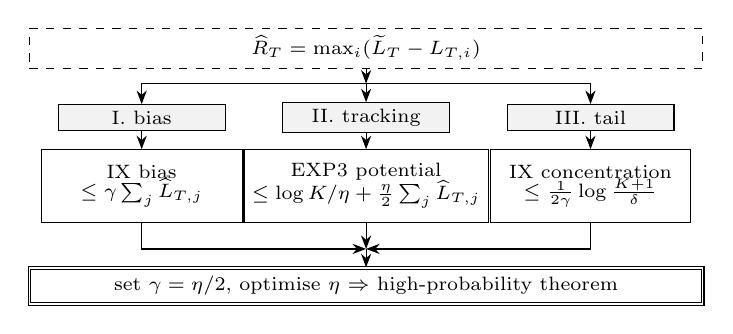
\begin{tikzpicture}[
  >=Stealth,
  font=\scriptsize,
  box/.style={draw,rectangle,align=center,inner sep=2.8pt,line width=0.38pt},
  tag/.style={draw,rectangle,align=center,inner sep=2.2pt,line width=0.38pt,fill=black!5},
  arr/.style={->,line width=0.42pt},
  dasharr/.style={->,dashed,line width=0.38pt}
]
  % Total horizontal span: 8.56cm, below the 9.4cm column width.
  \node[box,dashed,minimum width=8.55cm,minimum height=0.48cm] (goal) at (0,0)
    {$\Rhat_T=\max_i(\Ltil_T-L_{T,i})$};

  \coordinate (split) at (0,-0.45);
  \draw[arr] (goal.south) -- (split);

  \node[tag,minimum width=2.12cm] (b) at (-2.85,-0.88) {I. bias};
  \node[tag,minimum width=2.12cm] (t) at (0,-0.88) {II. tracking};
  \node[tag,minimum width=2.12cm] (c) at (2.85,-0.88) {III. tail};

  \draw[arr] (split) -| (b.north);
  \draw[arr] (split) -- (t.north);
  \draw[arr] (split) -| (c.north);

  \node[box,minimum width=2.55cm,minimum height=0.92cm] (lb) at (-2.85,-1.75)
    {IX bias\\[-1pt]$\le \gamma\sum_j\Lhat_{T,j}$};
  \node[box,minimum width=2.55cm,minimum height=0.92cm] (lt) at (0,-1.75)
    {EXP3 potential\\[-1pt]$\le \log K/\eta+\frac{\eta}{2}\sum_j\Lhat_{T,j}$};
  \node[box,minimum width=2.55cm,minimum height=0.92cm] (lc) at (2.85,-1.75)
    {IX concentration\\[-1pt]$\le \frac{1}{2\gamma}\log\frac{K+1}{\delta}$};

  \draw[arr] (b.south) -- (lb.north);
  \draw[arr] (t.south) -- (lt.north);
  \draw[arr] (c.south) -- (lc.north);

  \coordinate (join) at (0,-2.55);
  \draw[arr] (lb.south) |- (join);
  \draw[arr] (lt.south) -- (join);
  \draw[arr] (lc.south) |- (join);

  \node[box,double,double distance=0.55pt,minimum width=8.55cm,minimum height=0.46cm]
    (out) at (0,-3.02) {set $\gamma=\eta/2$, optimise $\eta$ $\Rightarrow$ high-probability theorem};
  \draw[arr] (join) -- (out.north);
\end{tikzpicture}
\finishcapsule

\capsule{09}{three local estimates}
\begin{tabularx}{\linewidth}{@{}>{\bfseries}lX@{}}
\toprule
Term & estimate used in the proof\\
\midrule
I & implicit exploration introduces a downward bias bounded by
$\gamma\sum_j\Lhat_{T,j}$; this is controlled by taking
$\gamma=O((TK)^{-1/2})$.\\[2pt]
II & exponential weights converts cumulative estimated loss into
$\log K/\eta+(\eta/2)\sum_j\Lhat_{T,j}$.\\[2pt]
III & the IX estimator admits a martingale tail bound because the
per-round estimate is capped by $1/\gamma$.\\
\bottomrule
\end{tabularx}
\finishcapsule

\capsule{10}{takeaway and references}
\begin{itemize}
  \item EXP3: unbiased estimator, expectation regret, high variance.
  \item EXP3-IX: biased estimator, capped estimates, high-probability regret.
  \item The price of concentration is the additive $\delta$-dependent tail.
\end{itemize}
\medskip
{\scriptsize
\textbf{[1]} P. Auer, N. Cesa-Bianchi, Y. Freund, R. Schapire. \emph{The Nonstochastic Multiarmed Bandit Problem}, 2002.\\
\textbf{[2]} G. Neu. \emph{Explore no more: Improved high-probability regret bounds for non-stochastic bandits}, 2015.\\
\textbf{[3]} T. Lattimore, C. Szepesvari. \emph{Bandit Algorithms}. Cambridge University Press, 2020.\\
\textbf{[4]} EE 290 Lecture 12 scribe notes, UC Berkeley, 2020.
}
\finishcapsule

\capsule{11}{symbol index}
{\scriptsize
\begin{tabularx}{\linewidth}{@{}>{\bfseries}lX>{\bfseries}lX@{}}
\toprule
$K$ & arms & $T$ & horizon\\
$P_t$ & sampling distribution & $A_t$ & sampled arm\\
$\eta$ & learning rate & $\gamma$ & implicit exploration\\
$\ellhat_{t,i}$ & IX estimator & $\Lhat_{t,i}$ & cumulative estimate\\
$\delta$ & failure probability & $\Rhat_T$ & random pseudo-regret\\
\bottomrule
\end{tabularx}}
\finishcapsule


\end{minipage}
\end{document}
